\documentclass[tikz,border=10pt]{standalone}
\usepackage{pgfplots}
\pgfplotsset{compat=1.18}
\usepgfplotslibrary{fillbetween}
\author{Jason Fan}
\begin{document}

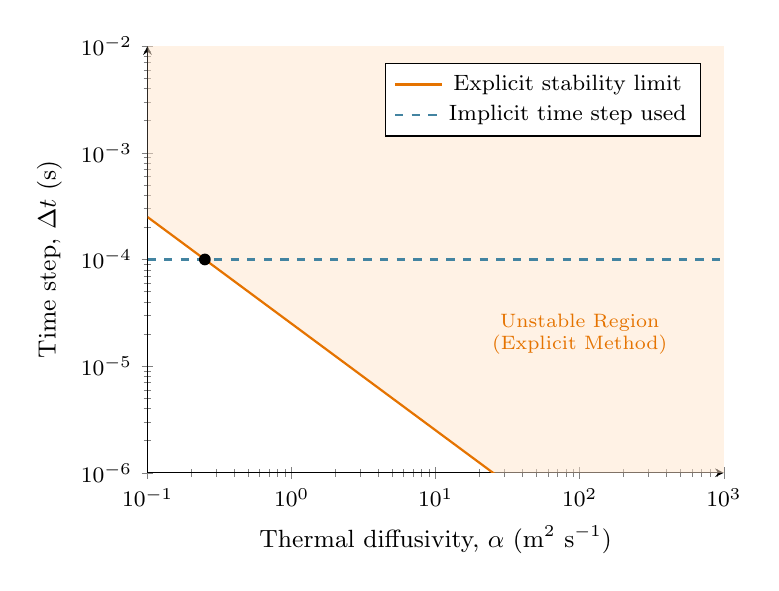
\begin{tikzpicture}
\begin{loglogaxis}[
    width=8.9cm,
    height=7cm,
    axis lines=left,
    grid=none,
    xmin=0.1, xmax=1000,
    ymin=1e-6, ymax=1e-2,
    xlabel={Thermal diffusivity, $\alpha$ (m$^2$ s$^{-1}$)},
    ylabel={Time step, $\Delta t$ (s)},
    label style={font=\small},
    tick label style={font=\footnotesize},
    legend style={
        draw=black,
        fill=white,
        at={(0.96,0.96)},
        anchor=north east,
        font=\footnotesize
    }
]

% dx = 0.01 => dx^2 = 0.0001)
\def\dxsq{0.0001}

% explicit
% dt = dx^2 / (4 * alpha)
\addplot[
    color=orange!90!black,
    thick,
    domain=0.1:1000,
    samples=200,
    name path=explicit
]
{\dxsq / (4 * x)};
\addlegendentry{Explicit stability limit}

% implicit and we use dt = 1e-4
\addplot[
    color=cyan!60!black,
    thick,
    dashed,
    domain=0.1:1000,
    samples=2,
    name path=implicit
]
{1e-4};
\addlegendentry{Implicit time step used}

% shade and stuff
\path[name path=top] (axis cs:0.1,1e-2) -- (axis cs:1000,1e-2);
\addplot[
    orange!20,
    opacity=0.5,
    forget plot
]
fill between[of=explicit and top];

\node[text=orange!90!black, font=\scriptsize, align=center] 
    at (axis cs: 100, 2e-5) {Unstable Region\\(Explicit Method)};

\node[circle, fill=black, inner sep=1.5pt] at (axis cs: 0.25, 1e-4) {};

\end{loglogaxis}
\end{tikzpicture}

\end{document}